\documentclass[twoside]{book}

% Packages required by doxygen
\usepackage{fixltx2e}
\usepackage{calc}
\usepackage{doxygen}
\usepackage[export]{adjustbox} % also loads graphicx
\usepackage{graphicx}
\usepackage[utf8]{inputenc}
\usepackage{makeidx}
\usepackage{multicol}
\usepackage{multirow}
\PassOptionsToPackage{warn}{textcomp}
\usepackage{textcomp}
\usepackage[nointegrals]{wasysym}
\usepackage[table]{xcolor}

% Font selection
\usepackage[T1]{fontenc}
\usepackage[scaled=.90]{helvet}
\usepackage{courier}
\usepackage{amssymb}
\usepackage{sectsty}
\renewcommand{\familydefault}{\sfdefault}
\allsectionsfont{%
  \fontseries{bc}\selectfont%
  \color{darkgray}%
}
\renewcommand{\DoxyLabelFont}{%
  \fontseries{bc}\selectfont%
  \color{darkgray}%
}
\newcommand{\+}{\discretionary{\mbox{\scriptsize$\hookleftarrow$}}{}{}}

% Page & text layout
\usepackage{geometry}
\geometry{%
  a4paper,%
  top=2.5cm,%
  bottom=2.5cm,%
  left=2.5cm,%
  right=2.5cm%
}
\tolerance=750
\hfuzz=15pt
\hbadness=750
\setlength{\emergencystretch}{15pt}
\setlength{\parindent}{0cm}
\setlength{\parskip}{3ex plus 2ex minus 2ex}
\makeatletter
\renewcommand{\paragraph}{%
  \@startsection{paragraph}{4}{0ex}{-1.0ex}{1.0ex}{%
    \normalfont\normalsize\bfseries\SS@parafont%
  }%
}
\renewcommand{\subparagraph}{%
  \@startsection{subparagraph}{5}{0ex}{-1.0ex}{1.0ex}{%
    \normalfont\normalsize\bfseries\SS@subparafont%
  }%
}
\makeatother

% Headers & footers
\usepackage{fancyhdr}
\pagestyle{fancyplain}
\fancyhead[LE]{\fancyplain{}{\bfseries\thepage}}
\fancyhead[CE]{\fancyplain{}{}}
\fancyhead[RE]{\fancyplain{}{\bfseries\leftmark}}
\fancyhead[LO]{\fancyplain{}{\bfseries\rightmark}}
\fancyhead[CO]{\fancyplain{}{}}
\fancyhead[RO]{\fancyplain{}{\bfseries\thepage}}
\fancyfoot[LE]{\fancyplain{}{}}
\fancyfoot[CE]{\fancyplain{}{}}
\fancyfoot[RE]{\fancyplain{}{\bfseries\scriptsize Generated by Doxygen }}
\fancyfoot[LO]{\fancyplain{}{\bfseries\scriptsize Generated by Doxygen }}
\fancyfoot[CO]{\fancyplain{}{}}
\fancyfoot[RO]{\fancyplain{}{}}
\renewcommand{\footrulewidth}{0.4pt}
\renewcommand{\chaptermark}[1]{%
  \markboth{#1}{}%
}
\renewcommand{\sectionmark}[1]{%
  \markright{\thesection\ #1}%
}

% Indices & bibliography
\usepackage{natbib}
\usepackage[titles]{tocloft}
\setcounter{tocdepth}{3}
\setcounter{secnumdepth}{5}
\makeindex

% Hyperlinks (required, but should be loaded last)
\usepackage{ifpdf}
\ifpdf
  \usepackage[pdftex,pagebackref=true]{hyperref}
\else
  \usepackage[ps2pdf,pagebackref=true]{hyperref}
\fi
\hypersetup{%
  colorlinks=true,%
  linkcolor=blue,%
  citecolor=blue,%
  unicode%
}

% Custom commands
\newcommand{\clearemptydoublepage}{%
  \newpage{\pagestyle{empty}\cleardoublepage}%
}

\usepackage{caption}
\captionsetup{labelsep=space,justification=centering,font={bf},singlelinecheck=off,skip=4pt,position=top}

%===== C O N T E N T S =====

\begin{document}

% Titlepage & ToC
\hypersetup{pageanchor=false,
             bookmarksnumbered=true,
             pdfencoding=unicode
            }
\pagenumbering{alph}
\begin{titlepage}
\vspace*{7cm}
\begin{center}%
{\Large My Project }\\
\vspace*{1cm}
{\large Generated by Doxygen 1.8.13}\\
\end{center}
\end{titlepage}
\clearemptydoublepage
\pagenumbering{roman}
\tableofcontents
\clearemptydoublepage
\pagenumbering{arabic}
\hypersetup{pageanchor=true}

%--- Begin generated contents ---
\chapter{Data Structure Index}
\section{Data Structures}
Here are the data structures with brief descriptions\+:\begin{DoxyCompactList}
\item\contentsline{section}{\hyperlink{structbackground}{background} \\*Struct for background }{\pageref{structbackground}}{}
\end{DoxyCompactList}

\chapter{File Index}
\section{File List}
Here is a list of all documented files with brief descriptions\+:\begin{DoxyCompactList}
\item\contentsline{section}{{\bfseries game.\+h} }{\pageref{game_8h}}{}
\item\contentsline{section}{\hyperlink{haut__bas_8c}{haut\+\_\+bas.\+c} }{\pageref{haut__bas_8c}}{}
\item\contentsline{section}{\hyperlink{main_8c}{main.\+c} \\*Testing Program }{\pageref{main_8c}}{}
\end{DoxyCompactList}

\chapter{Data Structure Documentation}
\hypertarget{structCircle}{}\section{Circle Struct Reference}
\label{structCircle}\index{Circle@{Circle}}
\subsection*{Data Fields}
\begin{DoxyCompactItemize}
\item 
\mbox{\Hypertarget{structCircle_abceecd15b990054ddc30441cfcbb205d}\label{structCircle_abceecd15b990054ddc30441cfcbb205d}} 
int {\bfseries x}
\item 
\mbox{\Hypertarget{structCircle_a78aef28b3c176d14e8d25f8cd84e7dfd}\label{structCircle_a78aef28b3c176d14e8d25f8cd84e7dfd}} 
int {\bfseries y}
\item 
\mbox{\Hypertarget{structCircle_a071d166f8d58ab6f055cdbbf494b33ce}\label{structCircle_a071d166f8d58ab6f055cdbbf494b33ce}} 
float {\bfseries rayon}
\end{DoxyCompactItemize}


The documentation for this struct was generated from the following file\+:\begin{DoxyCompactItemize}
\item 
I\+A.\+h\end{DoxyCompactItemize}

\hypertarget{structobjet}{}\section{objet Struct Reference}
\label{structobjet}\index{objet@{objet}}


struct for enemy  




{\ttfamily \#include $<$I\+A.\+h$>$}



\subsection{Detailed Description}
struct for enemy 

The documentation for this struct was generated from the following file\+:\begin{DoxyCompactItemize}
\item 
I\+A.\+h\end{DoxyCompactItemize}

\hypertarget{structObjet}{}\section{Objet Struct Reference}
\label{structObjet}\index{Objet@{Objet}}


Collaboration diagram for Objet\+:
% FIG 0
\subsection*{Data Fields}
\begin{DoxyCompactItemize}
\item 
\mbox{\Hypertarget{structObjet_a0dac95199f82a456854968bfe257a14e}\label{structObjet_a0dac95199f82a456854968bfe257a14e}} 
S\+D\+L\+\_\+\+Surface $\ast$ {\bfseries img}
\item 
\mbox{\Hypertarget{structObjet_aa96c8e462a0637c98ab3c192e7f1806a}\label{structObjet_aa96c8e462a0637c98ab3c192e7f1806a}} 
S\+D\+L\+\_\+\+Rect {\bfseries pos}
\item 
\mbox{\Hypertarget{structObjet_a5ca2a21e73d9832faccdffca0466574f}\label{structObjet_a5ca2a21e73d9832faccdffca0466574f}} 
\hyperlink{structCircle}{Circle} {\bfseries c}
\item 
\mbox{\Hypertarget{structObjet_a22b5f8635c29778f8a669585ec6ed6fd}\label{structObjet_a22b5f8635c29778f8a669585ec6ed6fd}} 
S\+D\+L\+\_\+\+Rect {\bfseries pos\+\_\+text}
\end{DoxyCompactItemize}


The documentation for this struct was generated from the following file\+:\begin{DoxyCompactItemize}
\item 
I\+A.\+h\end{DoxyCompactItemize}

\chapter{File Documentation}
\hypertarget{IA_8c}{}\section{I\+A.\+c File Reference}
\label{IA_8c}\index{I\+A.\+c@{I\+A.\+c}}
{\ttfamily \#include $<$stdio.\+h$>$}\newline
{\ttfamily \#include $<$stdlib.\+h$>$}\newline
{\ttfamily \#include $<$math.\+h$>$}\newline
{\ttfamily \#include $<$S\+D\+L/\+S\+D\+L.\+h$>$}\newline
{\ttfamily \#include $<$S\+D\+L/\+S\+D\+L\+\_\+image.\+h$>$}\newline
{\ttfamily \#include $<$S\+D\+L/\+S\+D\+L\+\_\+ttf.\+h$>$}\newline
{\ttfamily \#include \char`\"{}I\+A.\+h\char`\"{}}\newline
Include dependency graph for I\+A.\+c\+:

\hypertarget{main_8c}{}\section{main.\+c File Reference}
\label{main_8c}\index{main.\+c@{main.\+c}}
{\ttfamily \#include $<$stdlib.\+h$>$}\\*
{\ttfamily \#include $<$stdio.\+h$>$}\\*
{\ttfamily \#include $<$S\+D\+L/\+S\+D\+L.\+h$>$}\\*
{\ttfamily \#include $<$S\+D\+L/\+S\+D\+L\+\_\+image.\+h$>$}\\*
{\ttfamily \#include \char`\"{}background.\+h\char`\"{}}\\*
Include dependency graph for main.\+c\+:\nopagebreak
\begin{figure}[H]
\begin{center}
\leavevmode
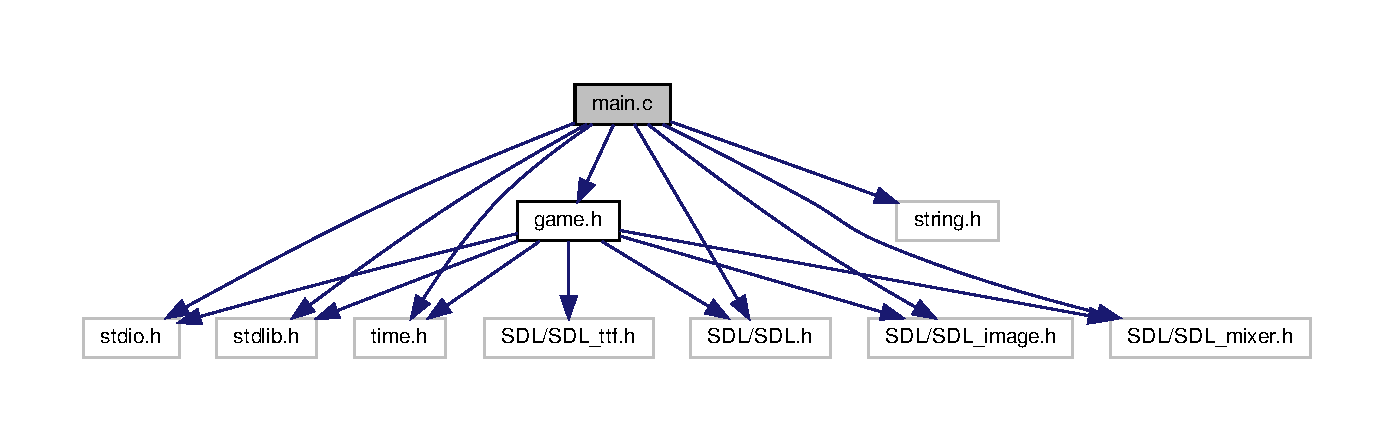
\includegraphics[width=350pt]{main_8c__incl}
\end{center}
\end{figure}
\subsection*{Functions}
\begin{DoxyCompactItemize}
\item 
int {\bfseries main} (int argc, char $\ast$argv\mbox{[}$\,$\mbox{]})\hypertarget{main_8c_a0ddf1224851353fc92bfbff6f499fa97}{}\label{main_8c_a0ddf1224851353fc92bfbff6f499fa97}

\end{DoxyCompactItemize}


\subsection{Detailed Description}
\begin{DoxyAuthor}{Author}
wael 
\end{DoxyAuthor}
\begin{DoxyDate}{Date}
Mai 14, 2020 
\end{DoxyDate}

%--- End generated contents ---

% Index
\backmatter
\newpage
\phantomsection
\clearemptydoublepage
\addcontentsline{toc}{chapter}{Index}
\printindex

\end{document}
